\chapter{Implementação} \label{cap:implementacao}

Este capítulo descreve a materialização do projeto \textbf{Karaokê Apache} em software. Considerando que o projeto encontra-se atualmente em \textbf{fase de Produto Mínimo Viável (MVP)}, as seções a seguir documentam o ambiente configurado, a estrutura da aplicação, os componentes já implementados e validados no núcleo funcional da Prova de Conceito (PoC/MVP), a integração entre a fila web e o reprodutor Electron, bem como os testes preliminares, resultados parciais e limitações próprias do estágio atual de desenvolvimento.

\section{Ambiente de Desenvolvimento}

O desenvolvimento e a execução do MVP foram conduzidos utilizando um ambiente padronizado entre os integrantes da equipe de desenvolvimento, composto pelos seguintes recursos de hardware, sistema operacional e ferramentas:

\begin{itemize}
  \item \textbf{Estações de Trabalho e Sistemas Operacionais:} computadores pessoais dos desenvolvedores e máquinas dos laboratórios de informática do IFSP -- Campus São Paulo, executando sistemas operacionais Windows 10/11 (64 bits) e distribuições Linux;
  \item \textbf{Linguagens, Banco de Dados e Ferramentas de Construção:} kit de desenvolvimento \textit{Java 21 (JDK 21)} para a API de back-end, Sistema de Gerenciamento de Banco de Dados \textit{MySQL}, ambiente \textit{Node.js} (com gerenciador de pacotes \texttt{npm}), empacotador \textit{Vite} e framework \textit{Electron} para o front-end e reprodutor de telão;
  \item \textbf{IDEs e Repositório de Código no GitHub:} desenvolvimento utilizando \textit{Visual Studio Code} / IDEs Java e versionamento distribuído centralizado no repositório oficial \url{https://github.com/MurilloAssis/Projeto-Extensao-Karaoke}.
\end{itemize}

\section{Estrutura da Aplicação}

A organização física de diretórios e pacotes da aplicação no estágio atual de MVP separa claramente o código do processo nativo do Electron, os componentes visuais em React e a camada de serviços/estado da fila. O Quadro \ref{quad:pacotes} apresenta o \textbf{Diagrama de Pacotes UML} da estrutura implementada.

\Needspace{11.2cm}
\begin{caixa}{Diagrama de Pacotes UML -- Estrutura de Diretórios e Módulos do MVP}{quad:pacotes}
\begin{center}
  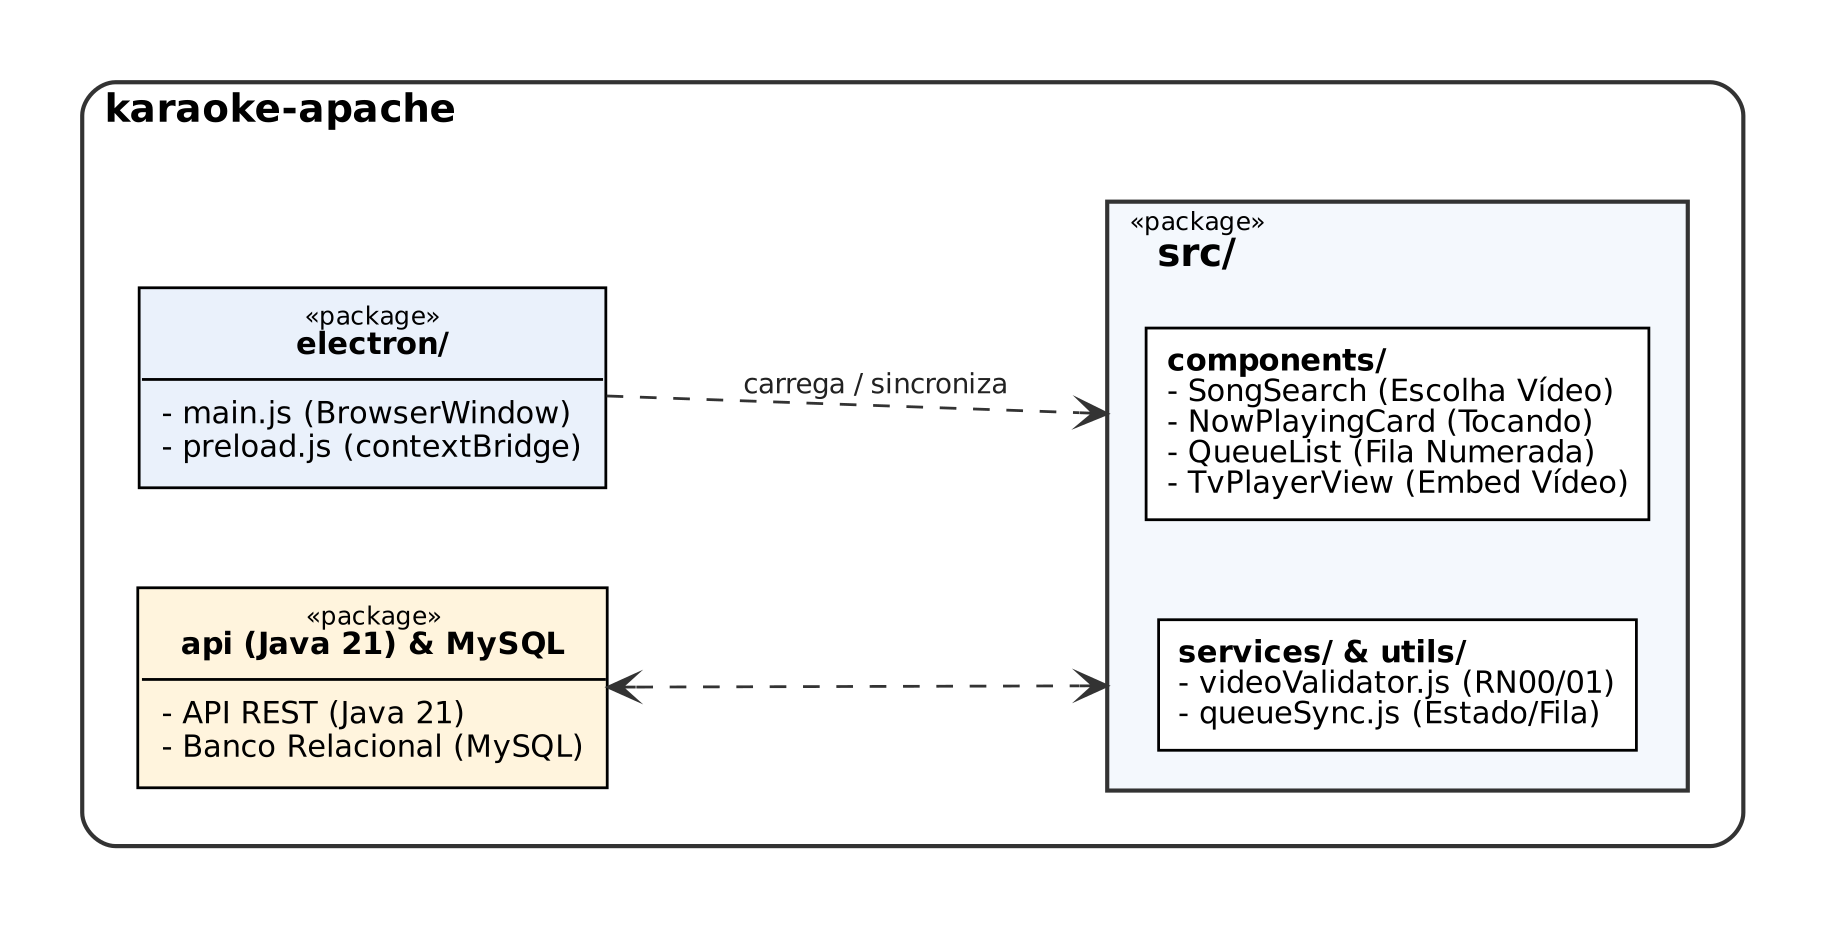
\includegraphics[width=\textwidth,height=0.78\textheight,keepaspectratio]{imagens/diagrama_pacotes.png}
\end{center}
\legend{Fonte: Elaborado pelos autores (2026).}
\end{caixa}

\section{Implementação dos Componentes}

Na fase atual de MVP, a implementação priorizou os componentes críticos responsáveis por validar a proposta central do sistema: receber pedidos musicais, organizar a fila sem duplicidades e controlar remotamente o que é reproduzido na TV do bar.

\begin{itemize}
  \item \textbf{Componente \textit{Pedido de Música}:} foi construído o módulo que permite a seleção de vídeos de karaokê pelo sistema e valida o identificador do vídeo escolhido. Caso o vídeo seja inválido/indisponível (RN00) ou o identificador já conste na fila ativa ou em reprodução (RN01), a inclusão na fila é bloqueada;
  \item \textbf{Componente \textit{Fila}:} foi implementada a gestão reativa da lista de músicas (\texttt{queue}) e da faixa ativa (\texttt{currentSong}). A interface permite adicionar itens ao final da fila, acionar o botão \textbf{Play} em qualquer posição, avançar para a \textbf{Próxima música} (promovendo automaticamente o primeiro item da fila para reprodução), excluir itens individuais e limpar toda a fila;
  \item \textbf{Componente \textit{Reprodutor} -- \textit{Karaokê TV Player}:} foi implementado o processo principal do Electron (\texttt{main.js}) que instancia uma janela dedicada (\texttt{BrowserWindow}) conectada ao estado da fila. Sempre que o estado de \texttt{currentSong} é atualizado na interface de controle, o \textit{Karaokê TV Player} exibe o código da faixa no cabeçalho (\textit{``Conectado -- Tocando: [ID]''}) e renderiza o player de vídeo do YouTube;
  \item \textbf{Componente \textit{Usuários} e Persistência Relacional (Java 21 e MySQL):} compreende a estruturação da API em Java 21 integrada ao banco de dados MySQL (\texttt{Conceitual.brM3}) para gerenciamento das entidades \texttt{usuario} (\texttt{admin}/\texttt{cliente}), \texttt{musica}, \texttt{letra} e \texttt{fila}.
\end{itemize}

\section{Integração dos Módulos}

Em ambiente de execução, os módulos da aplicação comunicam-se na mesma rede local do estabelecimento: o servidor web disponibiliza a interface de controle e fila em React/Vite (\texttt{http://localhost:5173}), enquanto a instância do aplicativo desktop \textbf{Karaokê TV Player} em Electron permanece aberta na saída de vídeo secundária conectada ao telão do palco. Qualquer ação de adição ou troca de música efetuada no controlador web propaga-se instantaneamente para a janela do Electron. O Quadro \ref{quad:implantacao} apresenta o \textbf{Diagrama de Implantação UML} que ilustra a topologia física de execução da solução no Apache Gru Rock Bar.

\Needspace{7.9cm}
\begin{caixa}{Diagrama de Implantação UML -- Topologia de Execução no Apache Gru Rock Bar}{quad:implantacao}
\begin{center}
  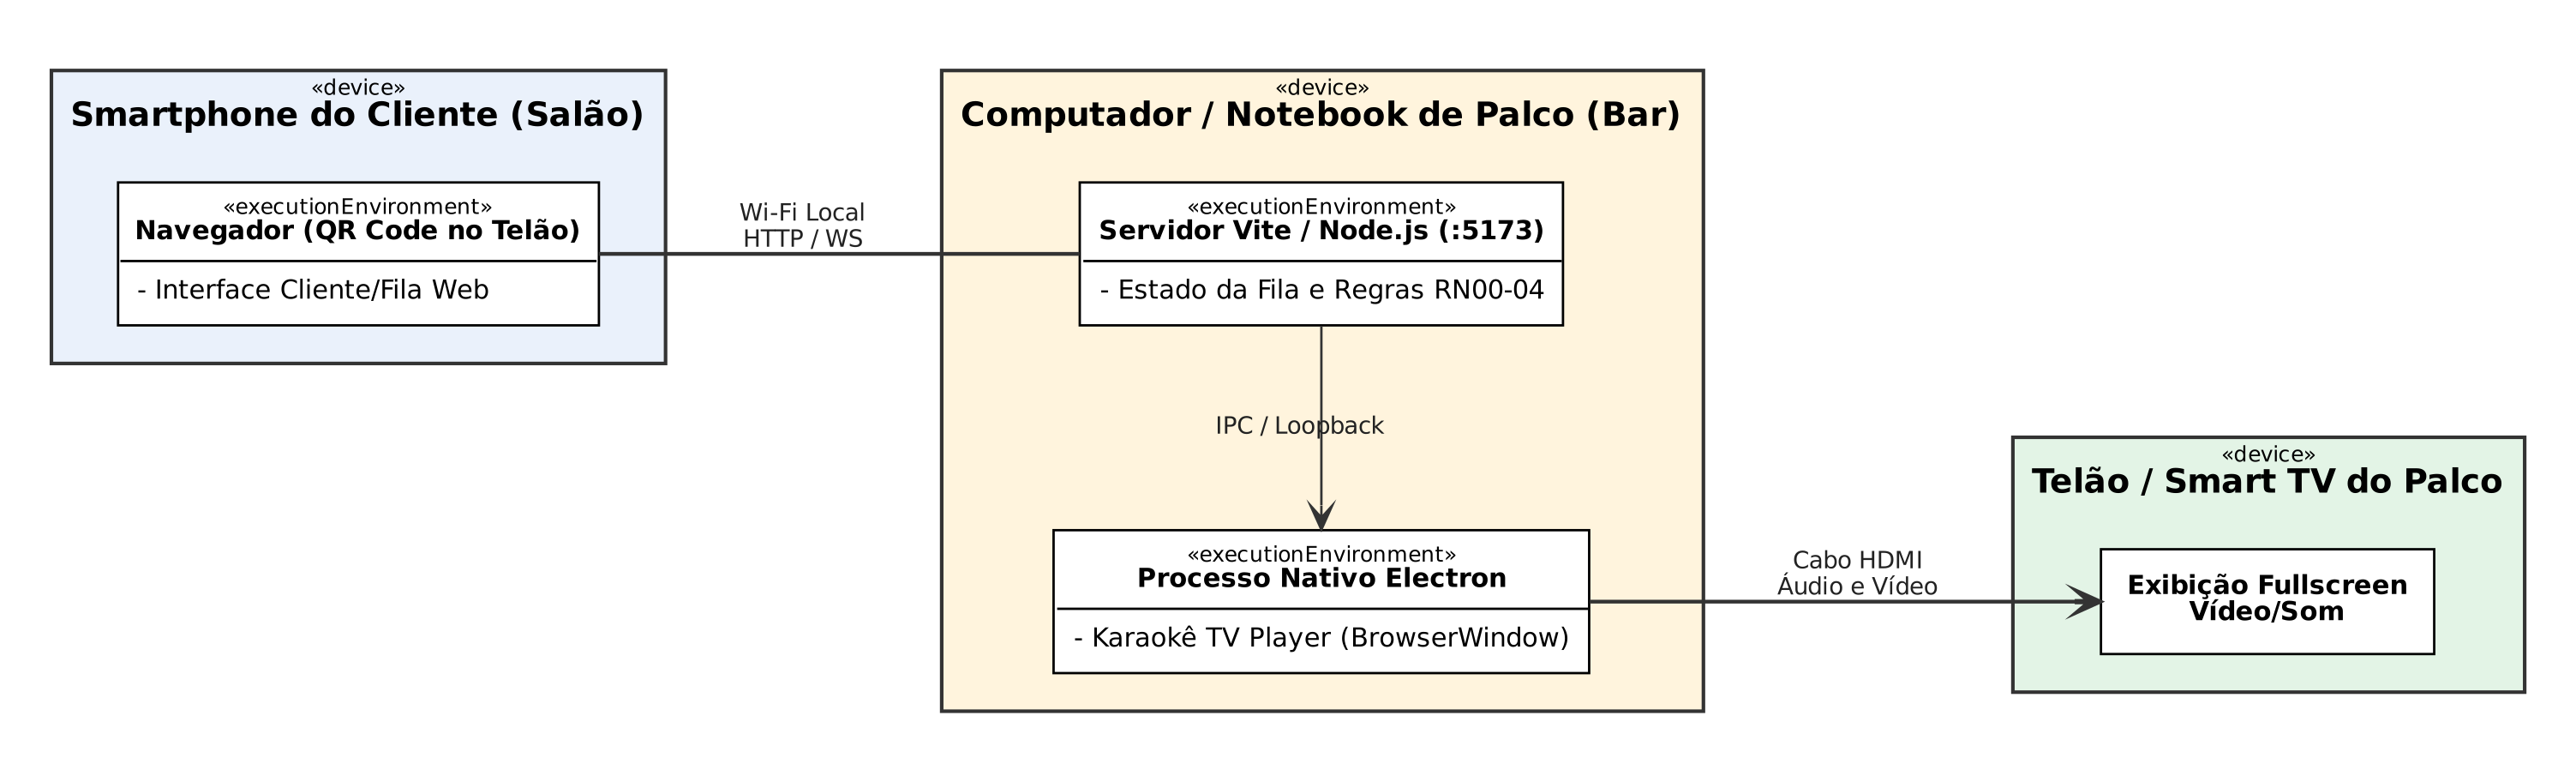
\includegraphics[width=\textwidth,height=0.78\textheight,keepaspectratio]{imagens/diagrama_implantacao.png}
\end{center}
\legend{Fonte: Elaborado pelos autores (2026).}
\end{caixa}

\section{Testes Realizados}

Como o projeto encontra-se em estágio de MVP, os procedimentos de teste concentraram-se na validação prática dos fluxos essenciais implementados na Prova de Conceito (registrada no vídeo \texttt{Poc.mp4}) e na verificação do funcionamento do reprodutor Electron em diferentes ambientes de rede. A Tabela \ref{tab:testes_mvp} sumariza os testes realizados até o momento.

\begin{table}[H]
\IBGEtab{%
  \caption{Testes preliminares realizados sobre a Prova de Conceito e o MVP.}%
  \label{tab:testes_mvp}%
}{%
  \footnotesize
  \begin{tabularx}{\textwidth}{p{1.3cm}p{3.2cm}X p{2.2cm}}
    \toprule
    \textbf{ID} & \textbf{Aspecto Avaliado} & \textbf{Procedimento Executado e Resultado Observado} & \textbf{Situação no MVP} \\
    \midrule
    TST-01 & Escolha e Adição de Vídeo à Fila pelo Sistema & Seleção de vídeos de karaokê (como \textit{Still Loving You -- Scorpions}, ID \texttt{R2F\_hGwD26g}, e \textit{Oh! Darling -- The Beatles}) na interface web; os itens foram validados e listados corretamente na fila numerada. & Validado (\texttt{Poc.mp4}) \\
    \addlinespace
    TST-02 & Sincronização do Comando \textit{Play} com o Electron & Acionamento do botão \textit{Play} na interface web (\texttt{localhost:5173}); o \textit{Karaokê TV Player} em Electron atualizou imediatamente o status para \textit{Conectado -- Tocando} e iniciou o vídeo. & Validado (\texttt{Poc.mp4}) \\
    \addlinespace
    TST-03 & Avanço de Faixa (\textit{Próxima música}) e Limpeza & Acionamento do botão \textit{Próxima música} e exclusão de itens; a fila avançou corretamente na ordem FIFO e atualizou a tela do reprodutor. & Validado (\texttt{Poc.mp4}) \\
    \addlinespace
    TST-04 & Bloqueio de Música Duplicada na Fila (RN01) & Tentativa de inserção repetida de um vídeo já presente na fila ativa; o sistema bloqueou a duplicidade e preservou a integridade da fila. & Validado \\
    \addlinespace
    TST-05 & Integração da API Java 21 com o MySQL & Testes de persistência das entidades modeladas e autenticação por perfil (\texttt{admin}/\texttt{cliente}) no banco de dados MySQL. & Em andamento (MVP) \\
    \bottomrule
  \end{tabularx}%
}{%
  \fonte{Elaborado pelos autores (2026).}%
}
\end{table}

\section{Resultados Obtidos}

Até o presente estágio de MVP, os resultados alcançados confirmam a viabilidade técnica da arquitetura proposta e atendem ao propósito central que motivou o projeto junto ao Apache Gru Rock Bar:

\begin{itemize}
  \item \textbf{Validação prática da orquestração entre Web e Electron (\texttt{Poc.mp4}):} comprovou-se que o operador do bar pode gerenciar a fila de músicas em uma interface web limpa enquanto o aplicativo desktop \textbf{Karaokê TV Player} reproduz automaticamente os vídeos selecionados em uma janela independente dedicada à TV, eliminando a necessidade de procurar vídeos manualmente e arrastar abas para o telão;
  \item \textbf{Consolidação da arquitetura e das regras do negócio:} o levantamento junto ao parceiro resultou em um conjunto coerente de regras de negócio (RN00 a RN04), modelo de dados (\texttt{Conceitual.brM3}) e divisão modular em quatro componentes (\textit{Usuários}, \textit{Fila}, \textit{Pedido de Música} e \textit{Reprodutor});
  \item \textbf{Adequação econômica ao parceiro:} toda a pilha tecnológica validada no MVP opera com custo zero de licenciamento, podendo ser executada diretamente no equipamento já disponível no estabelecimento.
\end{itemize}

\section{Limitações da Implementação}

Por tratar-se de uma versão em fase de Produto Mínimo Viável (MVP), registram-se as seguintes limitações atuais e pontos conhecidos que orientam a continuidade imediata do desenvolvimento:

\begin{itemize}
  \item \textbf{Escopo parcial da persistência e autenticação na PoC inicial:} no recorte validado na PoC (\texttt{Poc.mp4}), a fila e o estado da música atual operam de forma reativa em sessão local para validar a comunicação com o Electron, estando o acoplamento completo das telas de login/cadastro com o banco de dados relacional em fase de finalização no MVP;
  \item \textbf{Restrições externas de incorporação (\textit{embed}) do YouTube:} alguns vídeos musicais específicos possuem bloqueio de reprodução em quadros externos definido pelos canais proprietários no YouTube; no estágio atual do MVP, caso um link com bloqueio seja inserido, o operador utiliza o botão \textit{Próxima música} para avançar imediatamente para a faixa seguinte;
  \item \textbf{Transição automática ao final do vídeo:} na versão inicial do protótipo, o avanço para a próxima música pode ser acionado manualmente pelo organizador no botão \textit{Próxima música} ao término dos aplausos no palco, prevendo-se o gatilho opcional de avanço automático via eventos da API de IFrame do YouTube (\texttt{onStateChange}) nos incrementos seguintes.
\end{itemize}

%% -------------------------------------------------------------------------- %%
